\documentclass[UTF8,zihao=-4]{ctexart}
\usepackage[a4paper,top=2.0cm,bottom=2.0cm,left=2.2cm,right=2.2cm]{geometry}
\usepackage{amsmath,amssymb,booktabs,tabularx,array}
\usepackage{graphicx,float,caption}
\usepackage{xcolor,listings,tcolorbox}
\usepackage{fancyhdr,lastpage}
\usepackage[hidelinks]{hyperref}

\definecolor{navy}{HTML}{183B63}
\definecolor{blue}{HTML}{2B6EAE}
\definecolor{green}{HTML}{2F8F49}
\definecolor{orange}{HTML}{DF7615}
\definecolor{purple}{HTML}{7651B5}
\definecolor{soft}{HTML}{F3F7FB}
\definecolor{line}{HTML}{C9D4DF}
\definecolor{codebg}{HTML}{F6F8FA}
\definecolor{headergray}{HTML}{777777}

\hypersetup{
  pdftitle={系统开发工具基础 - 第3周实验报告},
  pdfauthor={朱元清},
  colorlinks=true,
  linkcolor=blue,
  urlcolor=blue
}

\pagestyle{fancy}
\fancyhf{}
\fancyhead[L]{\small\color{headergray}系统开发工具基础}
\fancyhead[R]{\small\color{headergray}第 3 周实验报告}
\fancyfoot[C]{\small\color{headergray}第 \thepage\ 页 / 共 \pageref{LastPage} 页}
\setlength{\headheight}{24pt}
\addtolength{\topmargin}{-12pt}
\renewcommand{\headrulewidth}{0.5pt}
\renewcommand{\headrule}{\hbox to\headwidth{\color{line}\leaders\hrule height \headrulewidth\hfill}}

\lstdefinestyle{shell}{
  language=bash,
  basicstyle=\ttfamily\footnotesize,
  backgroundcolor=\color{codebg},
  frame=single,
  rulecolor=\color{line},
  breaklines=true,
  columns=fullflexible,
  keepspaces=true,
  showstringspaces=false,
  xleftmargin=0.3em,
  xrightmargin=0.3em,
  aboveskip=0.6em,
  belowskip=0.7em
}

\lstdefinestyle{python}{
  language=Python,
  basicstyle=\ttfamily\footnotesize,
  backgroundcolor=\color{codebg},
  frame=single,
  rulecolor=\color{line},
  breaklines=true,
  columns=fullflexible,
  keepspaces=true,
  showstringspaces=false,
  xleftmargin=0.3em,
  xrightmargin=0.3em,
  aboveskip=0.6em,
  belowskip=0.7em
}

\newtcolorbox{summarybox}[1]{
  colback=soft,
  colframe=blue,
  boxrule=0.7pt,
  arc=2mm,
  title={#1},
  fonttitle=\bfseries,
  coltitle=navy
}

\newcommand{\experimentbanner}[3]{
  \begin{tcolorbox}[
    colback=soft,
    colframe=navy,
    boxrule=1pt,
    arc=2mm,
    left=4mm,right=4mm,top=2.5mm,bottom=2.5mm]
    \begin{tabularx}{\textwidth}{>{\Large\bfseries\color{navy}}p{2.7cm}X}
      实验 #1 & {\large\bfseries\color{navy}#2}\quad{\normalsize（#3）}
    \end{tabularx}
  \end{tcolorbox}
}

\newcommand{\practicebanner}[2]{
  \begin{tcolorbox}[
    colback=soft,
    colframe=navy,
    boxrule=1pt,
    arc=2mm,
    left=4mm,right=4mm,top=2.5mm,bottom=2.5mm]
    \begin{tabularx}{\textwidth}{>{\Large\bfseries\color{navy}}p{2.7cm}X}
      实例 #1 & {\large\bfseries\color{navy}#2}
    \end{tabularx}
  \end{tcolorbox}
}

\captionsetup{font=small,labelfont=bf,labelsep=quad}
\setlength{\parindent}{2em}
\setlength{\parskip}{0.25em}

\begin{document}

\thispagestyle{fancy}
\vspace*{0.7cm}
\begin{center}
  {\fontsize{28}{34}\selectfont\bfseries 系统开发工具基础}\\[0.35cm]
  {\fontsize{22}{28}\selectfont 第 3 周实验报告}\\[1.0cm]
  {\Large 姓名：朱元清\qquad 学号：25020007193}\\[0.6cm]
  {\Large 2026 年 9 月 7 日}
\end{center}

\vspace{0.7cm}
\begin{tcolorbox}[
  colback=soft,
  colframe=navy,
  boxrule=0.8pt,
  arc=2mm,
  left=5mm,right=5mm,top=4mm,bottom=4mm]
  \centering
  \normalsize
  本报告记录第 3 周第 9 至第 12 题的实现与验证过程，内容覆盖 Python Wheel
  打包安装、测试驱动修复、协作信息改写，以及 PyTorch 线性回归训练。
\end{tcolorbox}

\vspace{0.65cm}
\begin{table}[H]
  \centering
  \caption{第 3 周实验完成情况}
  \renewcommand{\arraystretch}{1.35}
  \begin{tabularx}{0.94\textwidth}{cX>{\raggedright\arraybackslash}p{4.5cm}c}
    \toprule
    实验 & 主题 & 关键工具 & 状态 \\
    \midrule
    9  & 从源码构建并在干净环境安装 Wheel & Python、build、pip、venv & \textcolor{blue}{\checkmark\ 完成} \\
    10 & 编程智能体的可验证修复闭环 & unittest、argparse、Git diff & \textcolor{green}{\checkmark\ 完成} \\
    11 & 将协作材料改写为可执行信息 & Markdown、提交信息、代码评审 & \textcolor{orange}{\checkmark\ 完成} \\
    12 & 可复现的线性回归训练循环 & Python、PyTorch、SGD & \textcolor{purple}{\checkmark\ 完成} \\
    \bottomrule
  \end{tabularx}
\end{table}

\vfill
\experimentbanner{九}{从源码构建并在干净环境安装 Wheel}{Packaging and Shipping Code}
\newpage

\subsection*{实现与执行命令}
本题在 \texttt{q09} 中创建 \texttt{greetlab} 命令行包，项目名为
\texttt{greetlab-25020007193}，入口命令为 \texttt{sdt-greet}。

\begin{lstlisting}[style=shell]
mkdir -p src/greetlab
touch src/greetlab/__init__.py

python3 -m venv venv_build
source venv_build/bin/activate
pip install build
python -m build
deactivate

python3 -m venv venv_clean
source venv_clean/bin/activate
pip install dist/greetlab_25020007193-0.1.0-py3-none-any.whl
cd ..
sdt-greet --name 25020007193
\end{lstlisting}

\begin{figure}[H]
  \centering
  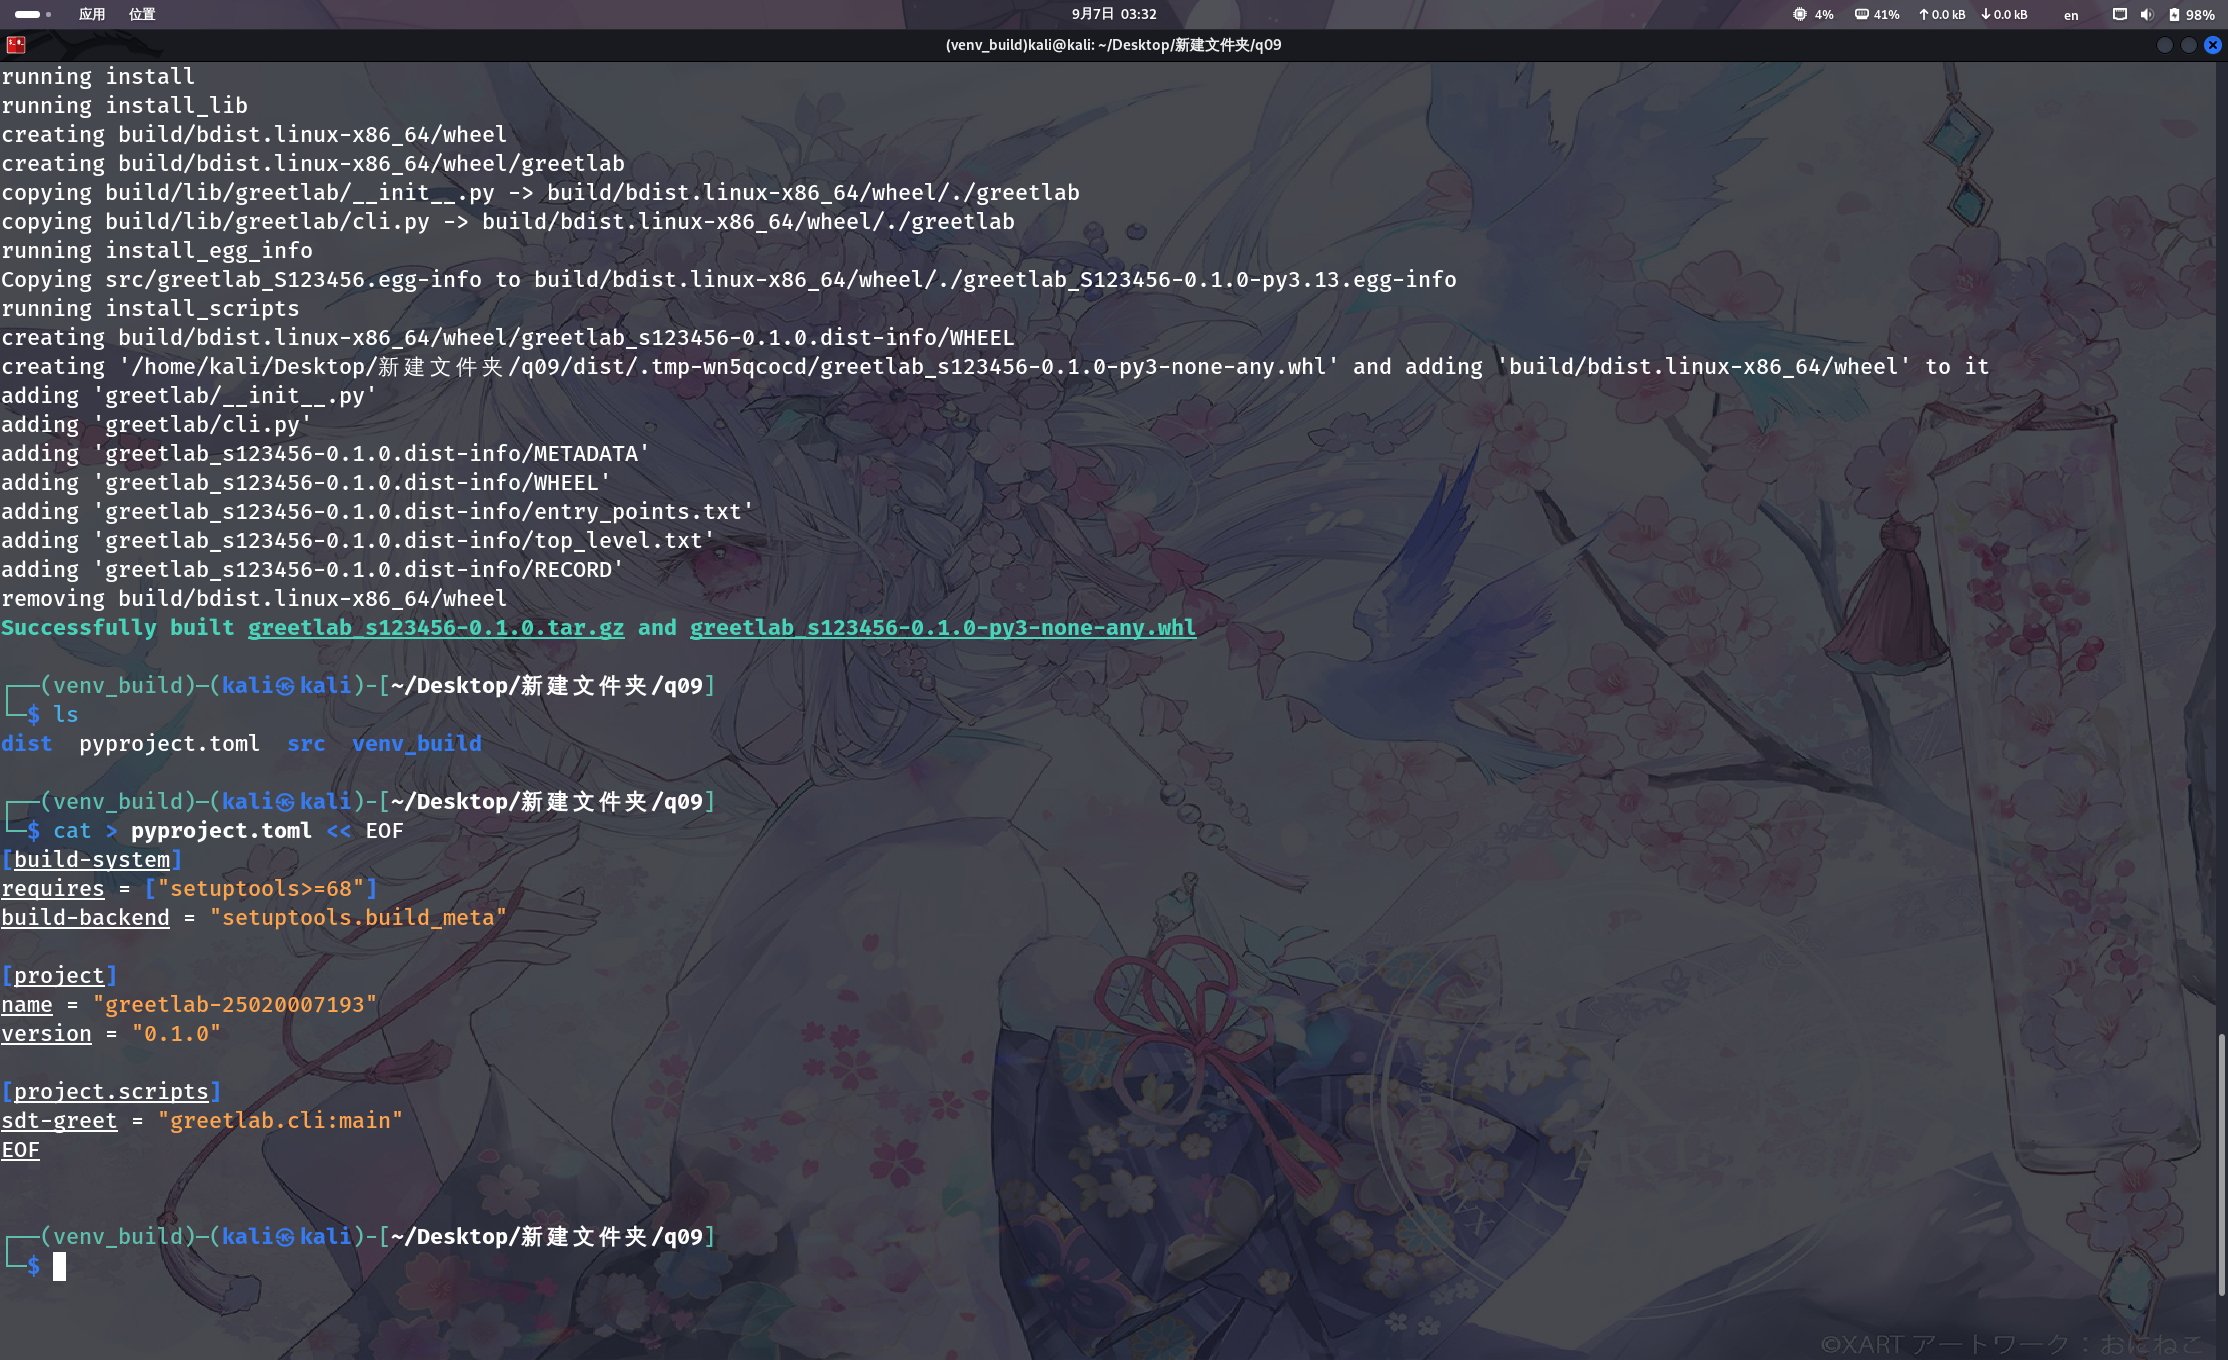
\includegraphics[width=.94\textwidth,height=.42\textheight,keepaspectratio]{assets/q09-build.png}
  \caption{实验九生成 Wheel 文件}
\end{figure}

\begin{figure}[H]
  \centering
  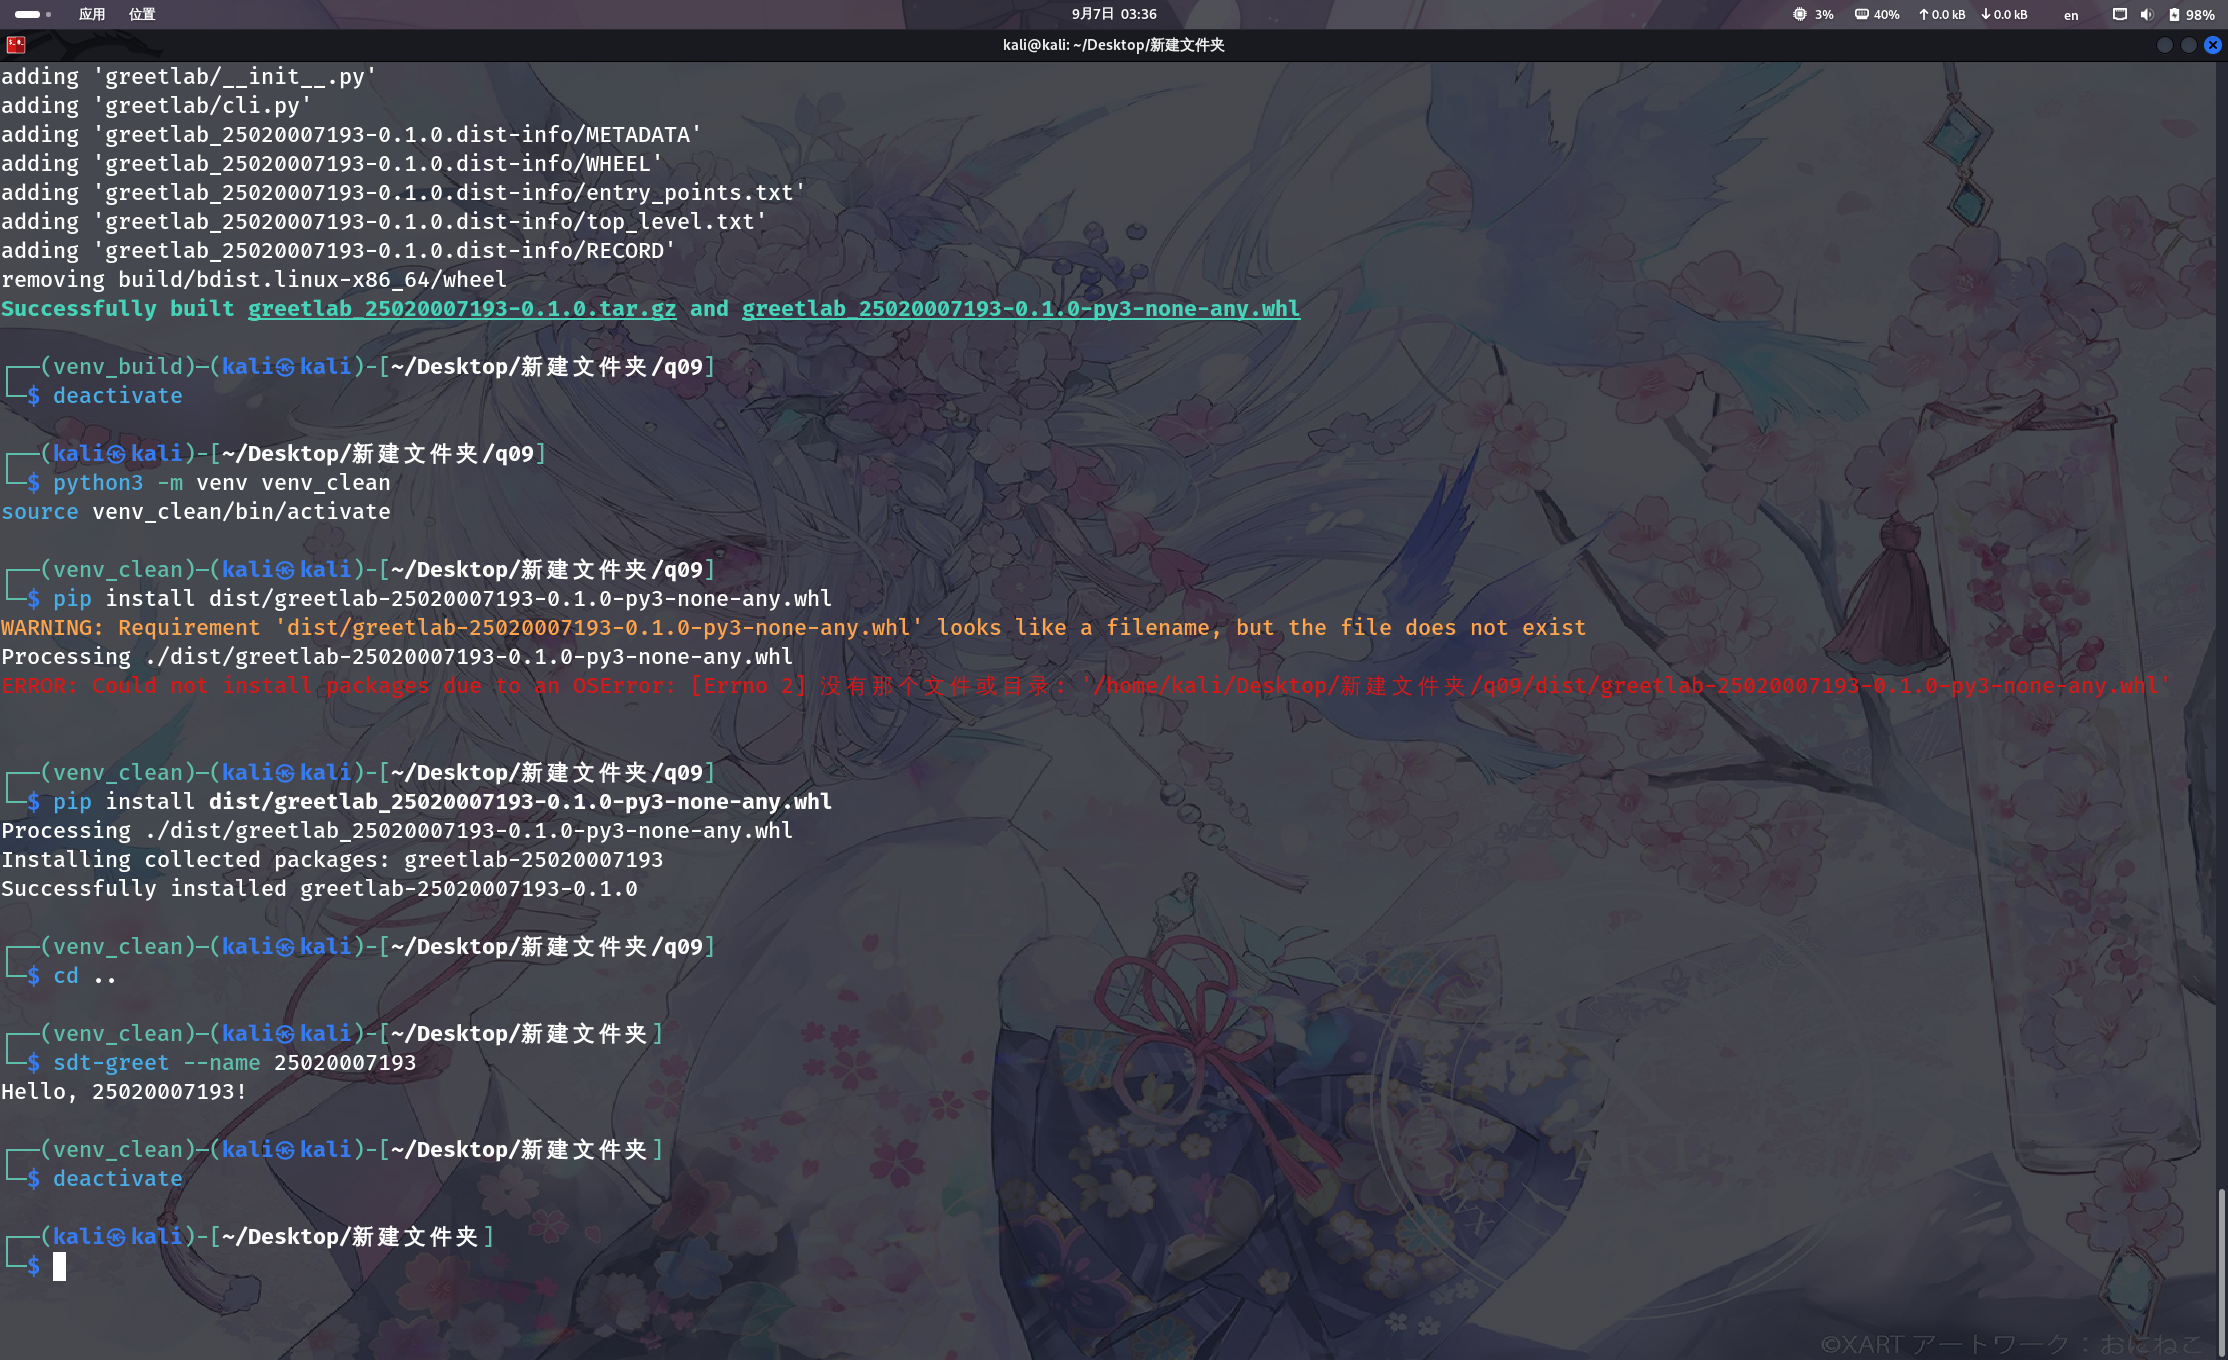
\includegraphics[width=.94\textwidth,height=.42\textheight,keepaspectratio]{assets/q09-install.png}
  \caption{实验九在干净虚拟环境安装并运行}
\end{figure}

\begin{summarybox}{结果说明}
\texttt{python -m build} 成功生成源代码包和 Wheel 文件。安装阶段第一次输入的
Wheel 文件名与实际生成文件不一致，提示文件不存在；随后改用
\texttt{greetlab\_25020007193-0.1.0-py3-none-any.whl} 完成安装。离开项目目录后执行
\texttt{sdt-greet --name 25020007193}，输出 \texttt{Hello, 25020007193!}，验证入口命令可用。
\end{summarybox}

\clearpage
\experimentbanner{十}{让编程智能体进入可验证的修复循环}{智能体编程}

\subsection*{失败测试与修复}
本题复用实验九的 \texttt{greetlab} 包。首先新增测试，要求 \texttt{--name} 仅包含
空白字符时 \texttt{main()} 抛出 \texttt{SystemExit(2)}。修复前测试失败；修复时仅在
参数解析后增加空白校验，并调用 \texttt{argparse} 的 \texttt{error()} 方法。

\begin{lstlisting}[style=python]
def main():
    p = argparse.ArgumentParser()
    p.add_argument("--name", required=True)
    a = p.parse_args()
    if not a.name.strip():
        p.error("--name must contain non-whitespace characters")
    print(f"Hello, {a.name}!")
\end{lstlisting}

\begin{lstlisting}[style=shell]
python -m unittest discover -s tests -v
python -c "import sys; sys.path.insert(0, 'src'); \
from greetlab.cli import main; \
sys.argv=['sdt-greet','--name','   ']; main()"
echo $LASTEXITCODE
git diff --no-index -- ../q09/q09/src/greetlab/cli.py src/greetlab/cli.py
\end{lstlisting}

\begin{figure}[H]
  \centering
  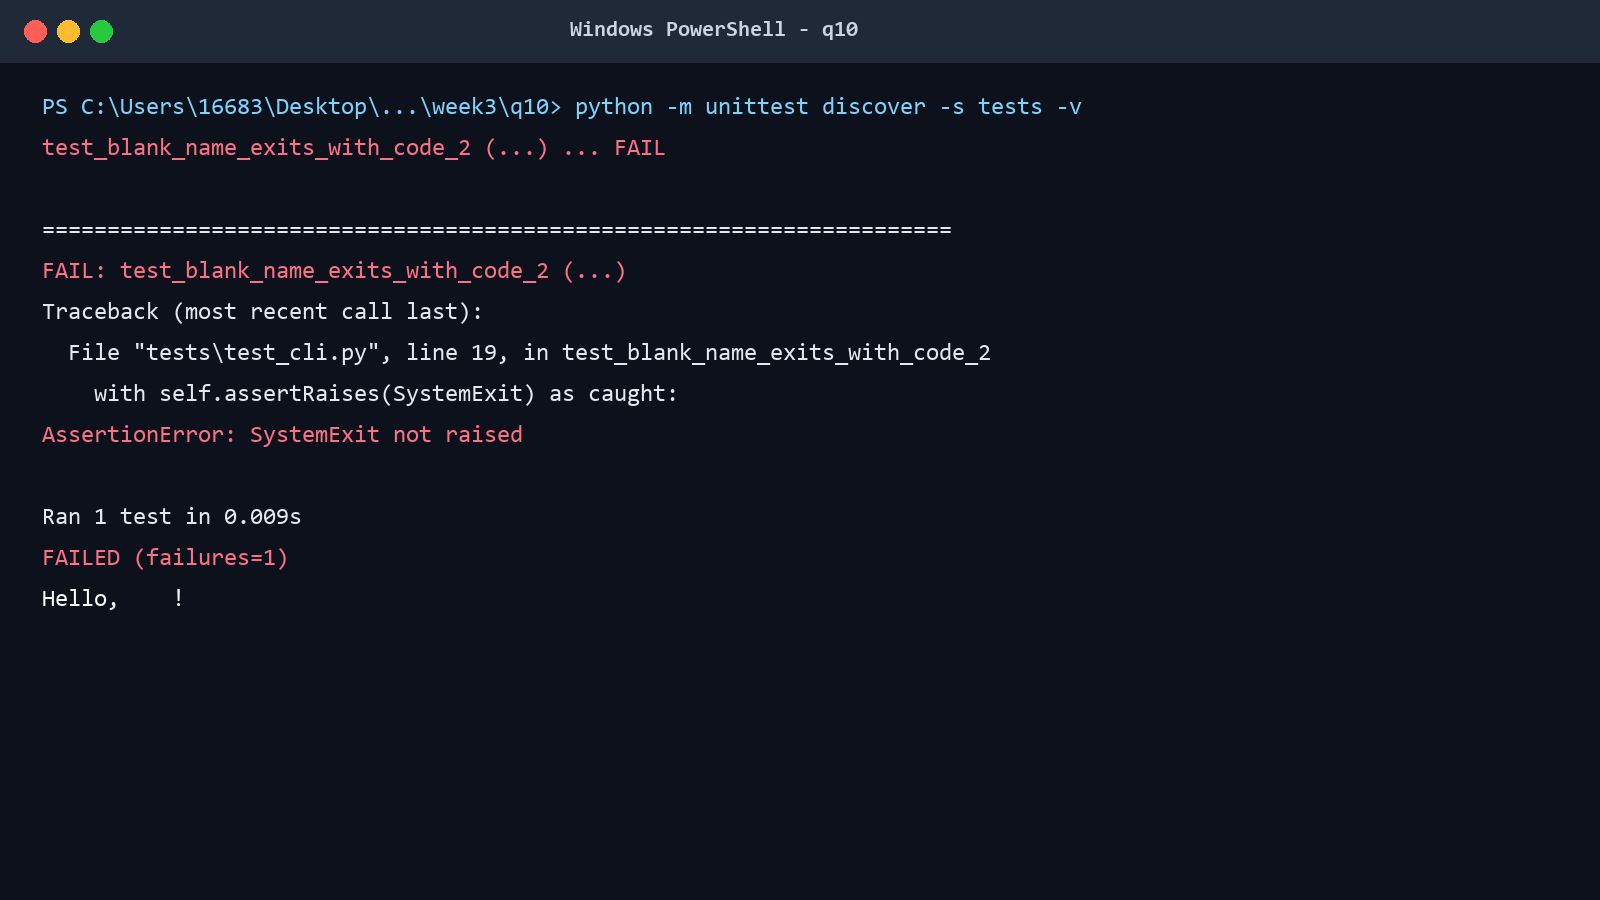
\includegraphics[width=.91\textwidth,height=.35\textheight,keepaspectratio]{assets/q10-failing-test.png}
  \caption{实验十修复前的失败测试}
\end{figure}

\begin{figure}[H]
  \centering
  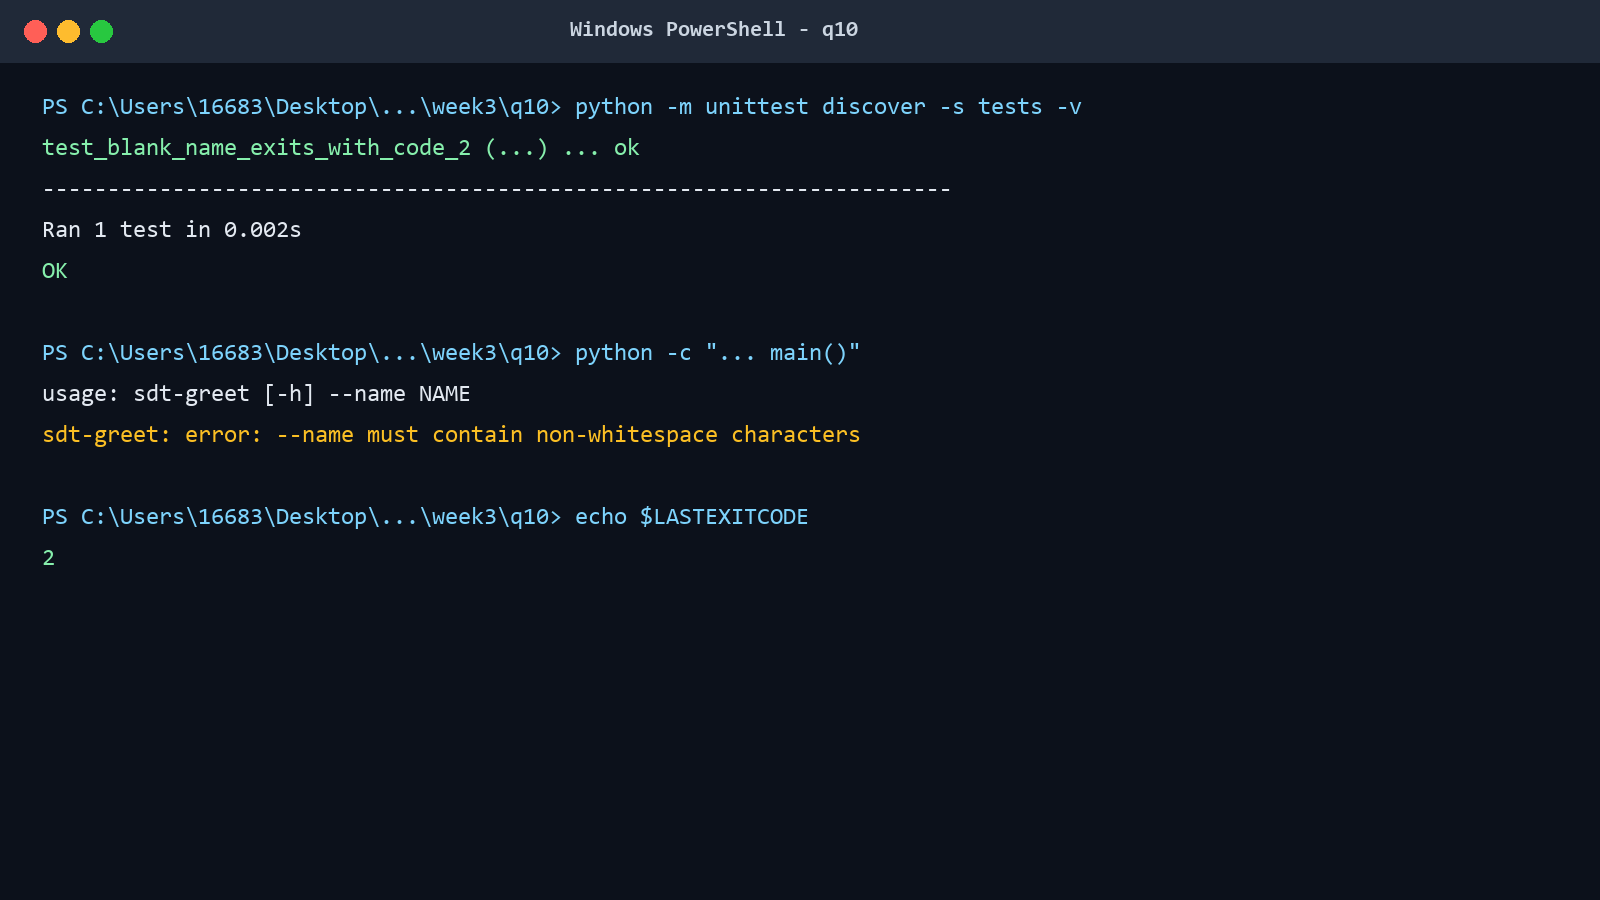
\includegraphics[width=.91\textwidth,height=.35\textheight,keepaspectratio]{assets/q10-passing-test.png}
  \caption{实验十修复后的测试与退出码验证}
\end{figure}

\begin{summarybox}{结果说明}
修复前测试报告 \texttt{SystemExit not raised}，原程序会输出空姓名问候语。修复后
单元测试通过，空白名称触发 argparse 错误并返回退出码 \texttt{2}。人工检查 diff 后，
确认代码只新增空白校验，没有无关改动。
\end{summarybox}

\clearpage
\experimentbanner{十一}{把无法处理的协作材料改成可执行信息}{不止于代码}

\subsection*{协作材料改写}
本题围绕“空姓名仍输出问候语”的缺陷，重写 \texttt{communication.md} 中的 Issue、
提交信息和评审意见。Issue 明确记录环境为待确认、复现命令、期望结果与实际结果；
提交信息说明问题原因和修改方向；评审意见采用 \texttt{Blocking} 标识风险与建议动作。

\begin{lstlisting}[style=shell]
# 查看改写后的协作材料
cat communication.md
\end{lstlisting}

\begin{figure}[H]
  \centering
  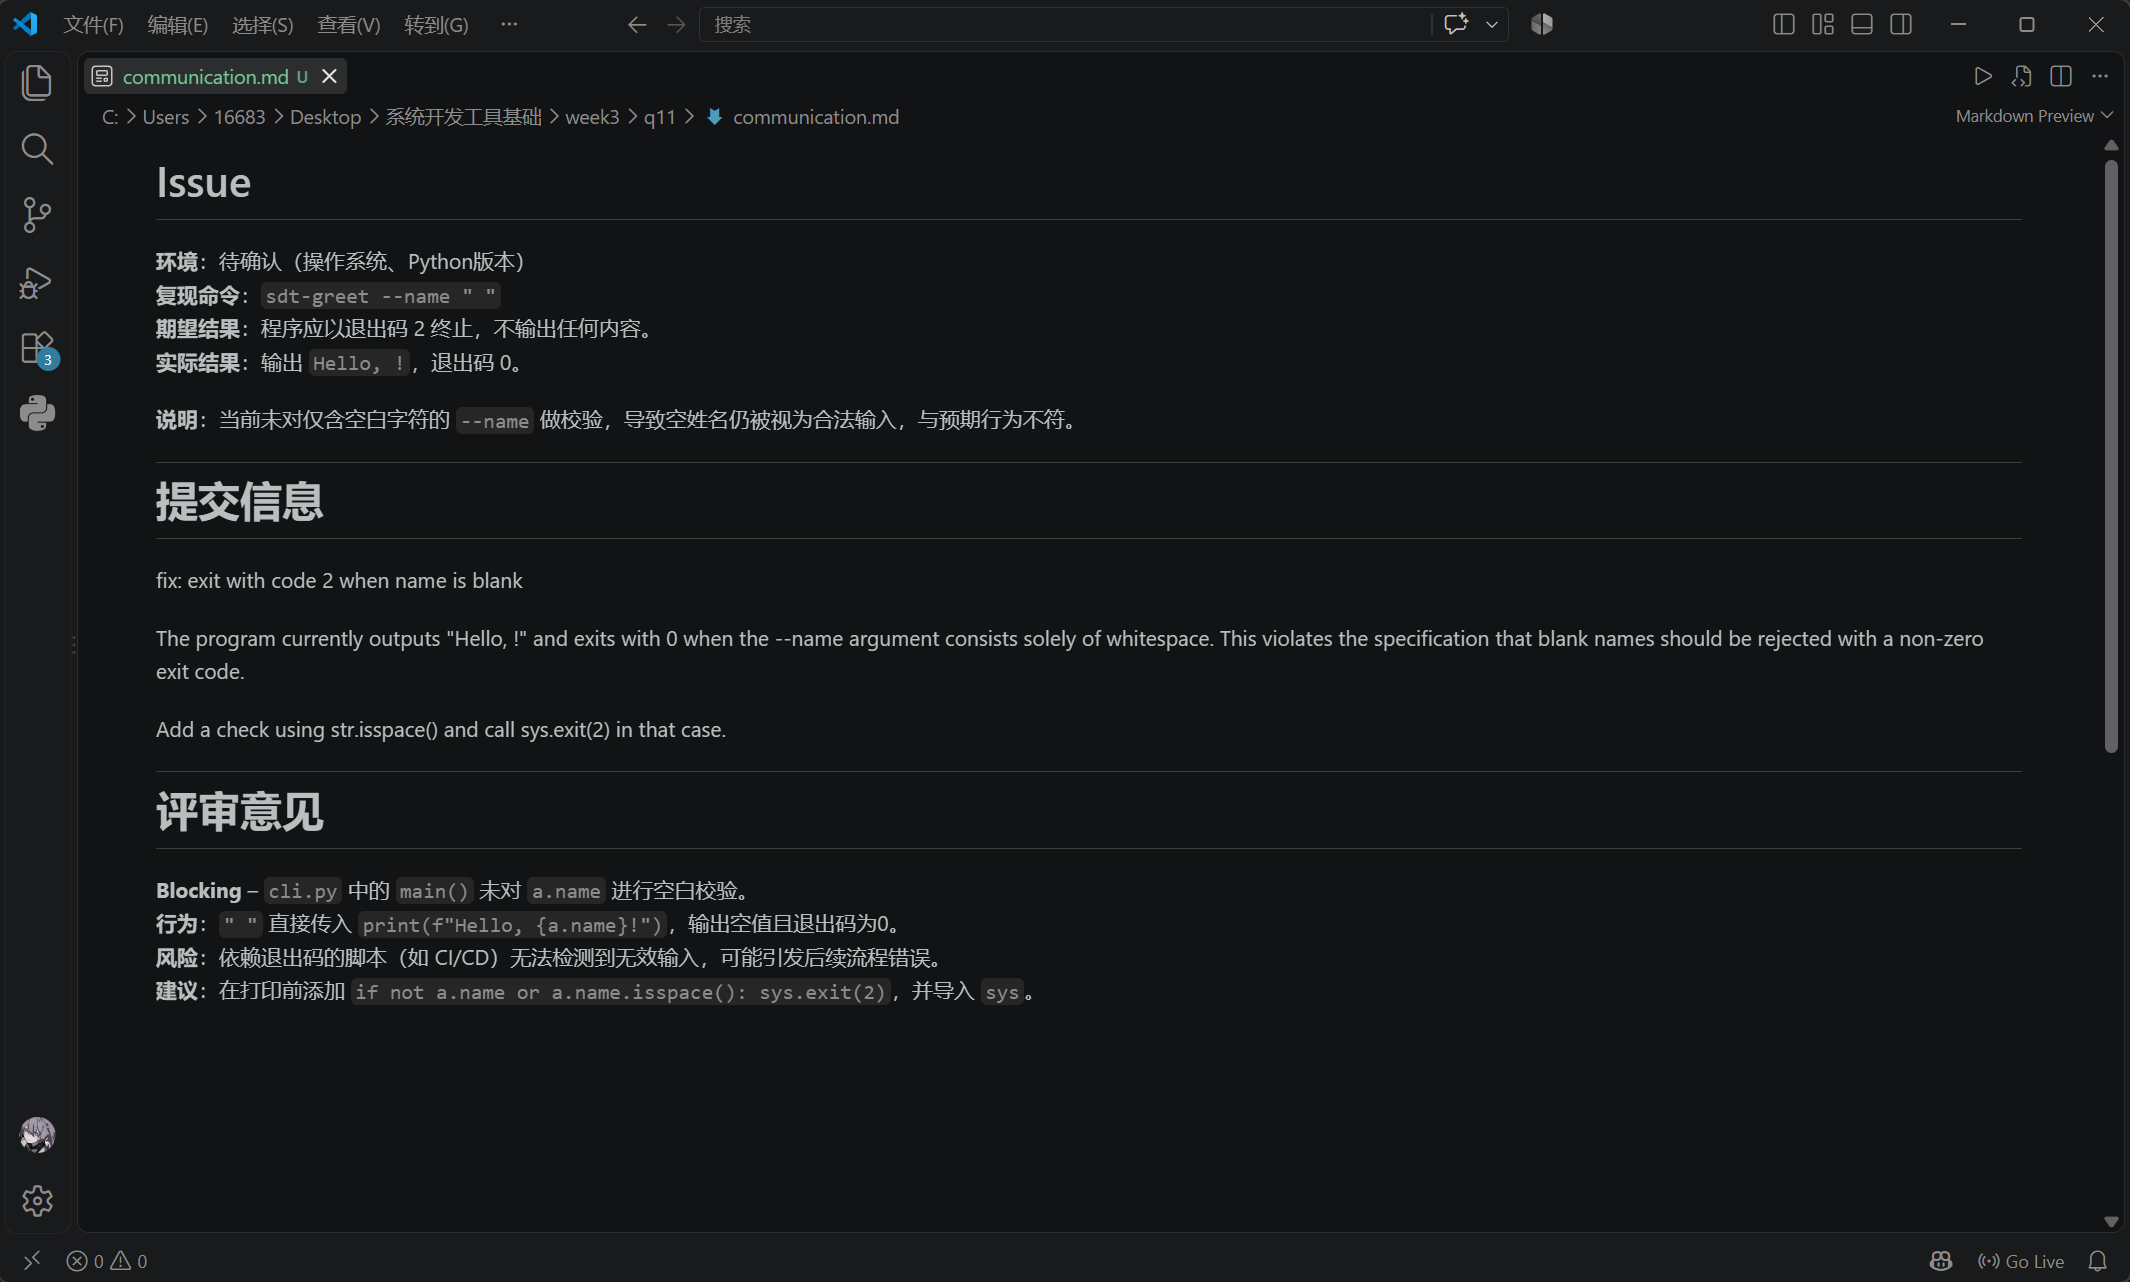
\includegraphics[width=.94\textwidth,height=.54\textheight,keepaspectratio]{assets/q11-communication.png}
  \caption{实验十一的可执行协作信息}
\end{figure}

\begin{summarybox}{结果说明}
改写后的 Issue 包含环境、复现命令、期望结果和实际结果，其中未知环境明确标为
“待确认”。提交信息使用祈使语气描述修复目标；评审意见说明了未校验空白输入的行为、
对依赖退出码脚本的风险，并给出带 \texttt{Blocking} 标记的具体修复建议。
\end{summarybox}

\clearpage
\experimentbanner{十二}{修复一个可复现的线性回归训练循环}{Python 与 PyTorch}

\subsection*{训练代码与执行}
训练数据满足线性关系 $y=3x-1$。使用固定随机种子，在线性层上以均方误差为损失函数、
SGD 为优化器完成 200 次 CPU 训练；随后切换为评估模式，在 \texttt{no\_grad()} 中计算
最终损失并输出参数。

\begin{lstlisting}[style=python]
torch.manual_seed(20260907)
x = torch.linspace(-1, 1, 101).reshape(-1, 1)
y = 3 * x - 1
model = nn.Linear(1, 1)
loss_fn = nn.MSELoss()
opt = torch.optim.SGD(model.parameters(), lr=0.1)

for _ in range(200):
    pred = model(x)
    loss = loss_fn(pred, y)
    opt.zero_grad()
    loss.backward()
    opt.step()

model.eval()
with torch.no_grad():
    final_loss = loss_fn(model(x), y)
    print(f"Final loss: {final_loss:.6f}")
    print(f"weight: {model.weight.item():.6f}")
    print(f"bias: {model.bias.item():.6f}")
\end{lstlisting}

\begin{lstlisting}[style=shell]
python train.py
\end{lstlisting}

\begin{summarybox}{结果说明}
训练结果显示最终损失为 \texttt{0.000000}，满足小于 \texttt{0.001} 的要求；
学习到的权重为 \texttt{2.999997}，偏置为 \texttt{-1.000000}，均接近目标关系
$y=3x-1$ 的参数，且未直接对参数赋值。
\end{summarybox}

\clearpage
\begin{figure}[H]
  \centering
  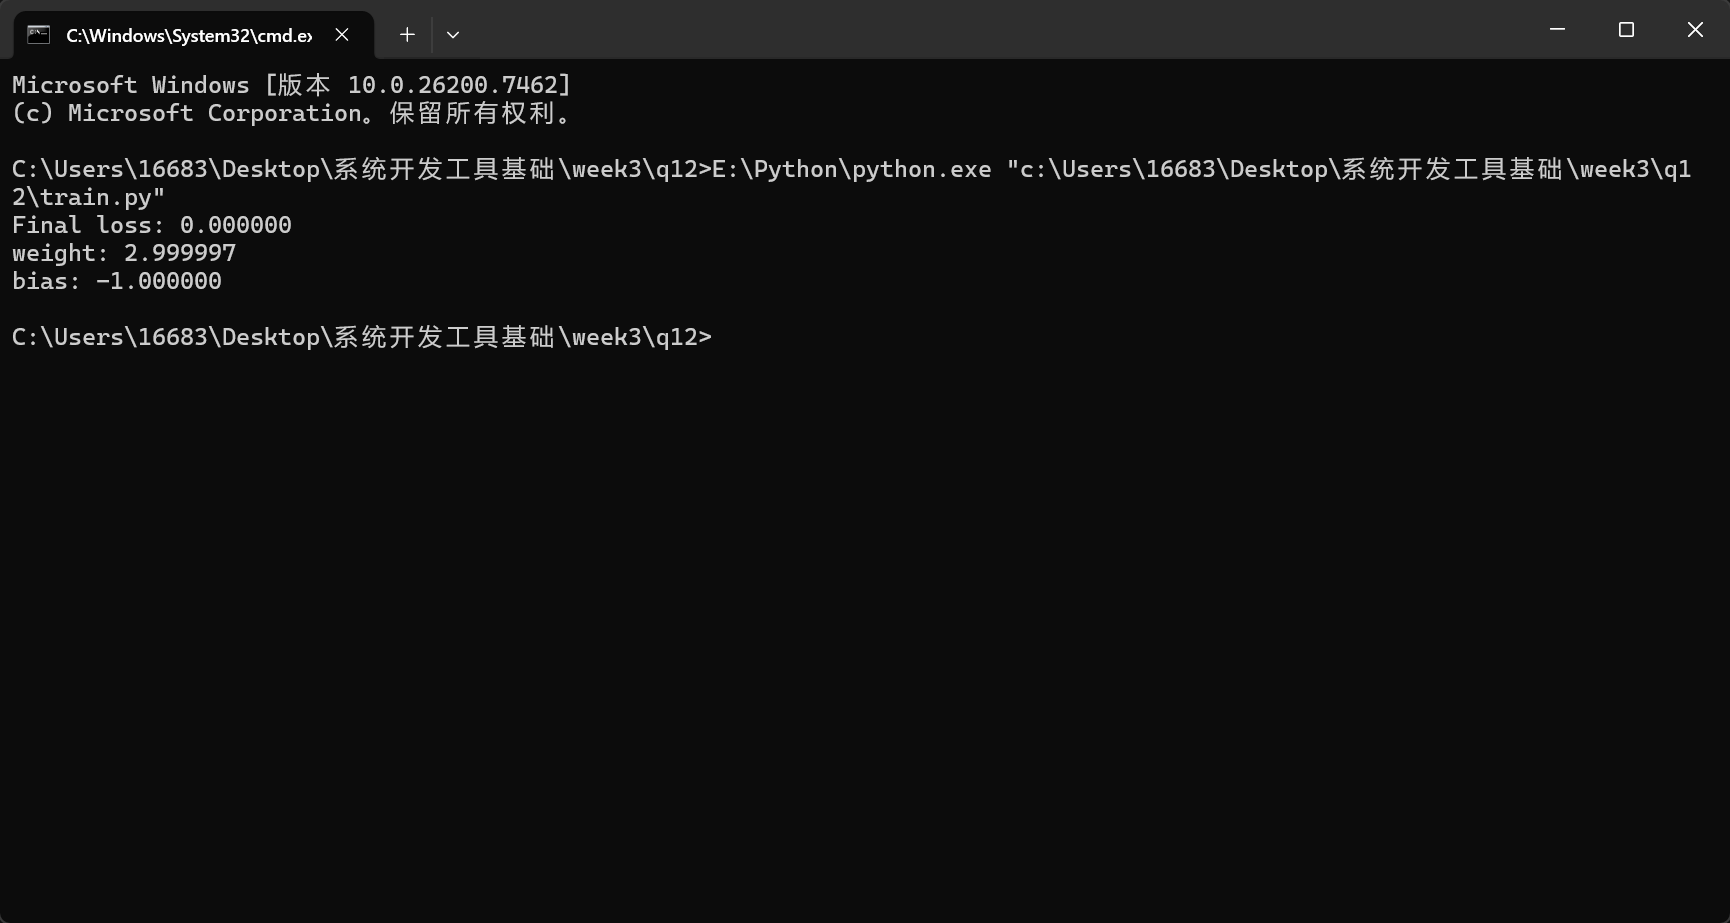
\includegraphics[width=.94\textwidth,height=.46\textheight,keepaspectratio]{assets/q12-run.png}
  \caption{实验十二的训练结果}
\end{figure}

\clearpage
\vspace*{0.9cm}
\begin{center}
  {\fontsize{26}{32}\selectfont\bfseries 课后练习}\\[0.35cm]
  {\Large Packaging and Shipping Code、智能体编程与不止于代码}
\end{center}

\vspace{0.7cm}
\begin{table}[H]
  \centering
  \caption{课后练习选题}
  \renewcommand{\arraystretch}{1.30}
  \begin{tabularx}{0.94\textwidth}{c>{\raggedright\arraybackslash}p{2.4cm}X>{\raggedright\arraybackslash}p{3.0cm}}
    \toprule
    编号 & 课程来源 & 实例内容 & 验证结果 \\
    \midrule
    1 & Shipping 1 & 虚拟环境前后环境变量对比 & PATH 与 VIRTUAL\_ENV 已变化 \\
    2 & Shipping 2 & Wheel 安装与依赖锁定记录 & 本地 Wheel 安装并成功运行 \\
    3 & Shipping 4 & Python 服务 Docker 配置 & Dockerfile 与 Compose 文件完成 \\
    4 & Agentic 1 & 四种编程方式体验比较 & 形成适用场景对比 \\
    5 & Agentic 2 & 智能体阅读陌生包 & 梳理入口与打包流程 \\
    6 & Agentic 3 & 氛围编程小应用 & 生成可打开的问候页 \\
    7 & Agentic 5 & 不直接编辑 Markdown & rg 提取全部无序列表项 \\
    8 & Beyond Code 2 & Git 提交信息对比 & 指出缺失的背景与影响 \\
    9 & Beyond Code 5 & 最小可复现示例 & 空白名称缺陷可稳定复现 \\
    10 & Beyond Code 3 & README 信息结构对比 & 总结漏斗式组织方式 \\
    \bottomrule
  \end{tabularx}
\end{table}

\clearpage
\practicebanner{1}{比较虚拟环境激活前后的环境变量}

\subsection*{执行命令}
\begin{lstlisting}[style=shell]
Get-ChildItem Env: | Sort-Object Name > before.txt
python -m venv .venv
. .\.venv\Scripts\Activate.ps1
Get-ChildItem Env: | Sort-Object Name > after.txt
Compare-Object (Get-Content before.txt) (Get-Content after.txt)
\end{lstlisting}

\begin{figure}[H]
  \centering
  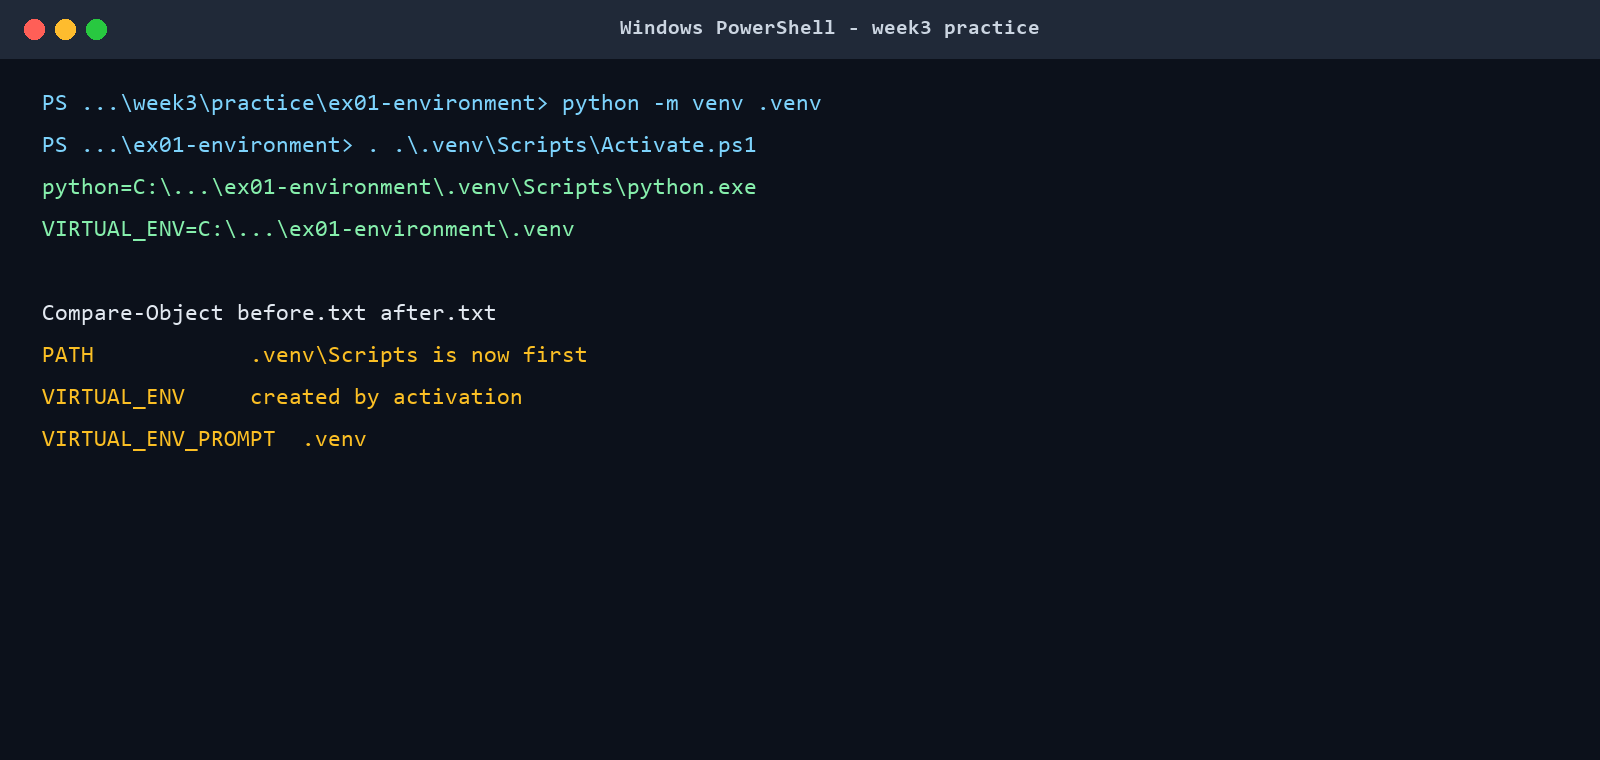
\includegraphics[width=.91\textwidth,height=.39\textheight,keepaspectratio]{assets/practice-ex01-env.png}
  \caption{实例 1 虚拟环境激活后的环境变化}
\end{figure}

\begin{summarybox}{结果说明}
激活后，解释器路径切换到 \texttt{.venv\textbackslash Scripts\textbackslash python.exe}，
\texttt{.venv\textbackslash Scripts} 被置于 \texttt{PATH} 的前部，同时新增
\texttt{VIRTUAL\_ENV} 与 \texttt{VIRTUAL\_ENV\_PROMPT}。因此 Shell 会优先定位虚拟环境中的
Python 与安装包，而不会污染系统级环境。
\end{summarybox}

\clearpage
\practicebanner{2}{从本地 Wheel 安装并生成锁定记录}

\subsection*{执行命令}
\begin{lstlisting}[style=shell]
python -m venv .venv
.\.venv\Scripts\pip install ..\..\q09\q09\dist\greetlab_25020007193-0.1.0-py3-none-any.whl
.\.venv\Scripts\sdt-greet.exe --name 25020007193
.\.venv\Scripts\python.exe -m pip freeze > requirements.lock
\end{lstlisting}

\begin{figure}[H]
  \centering
  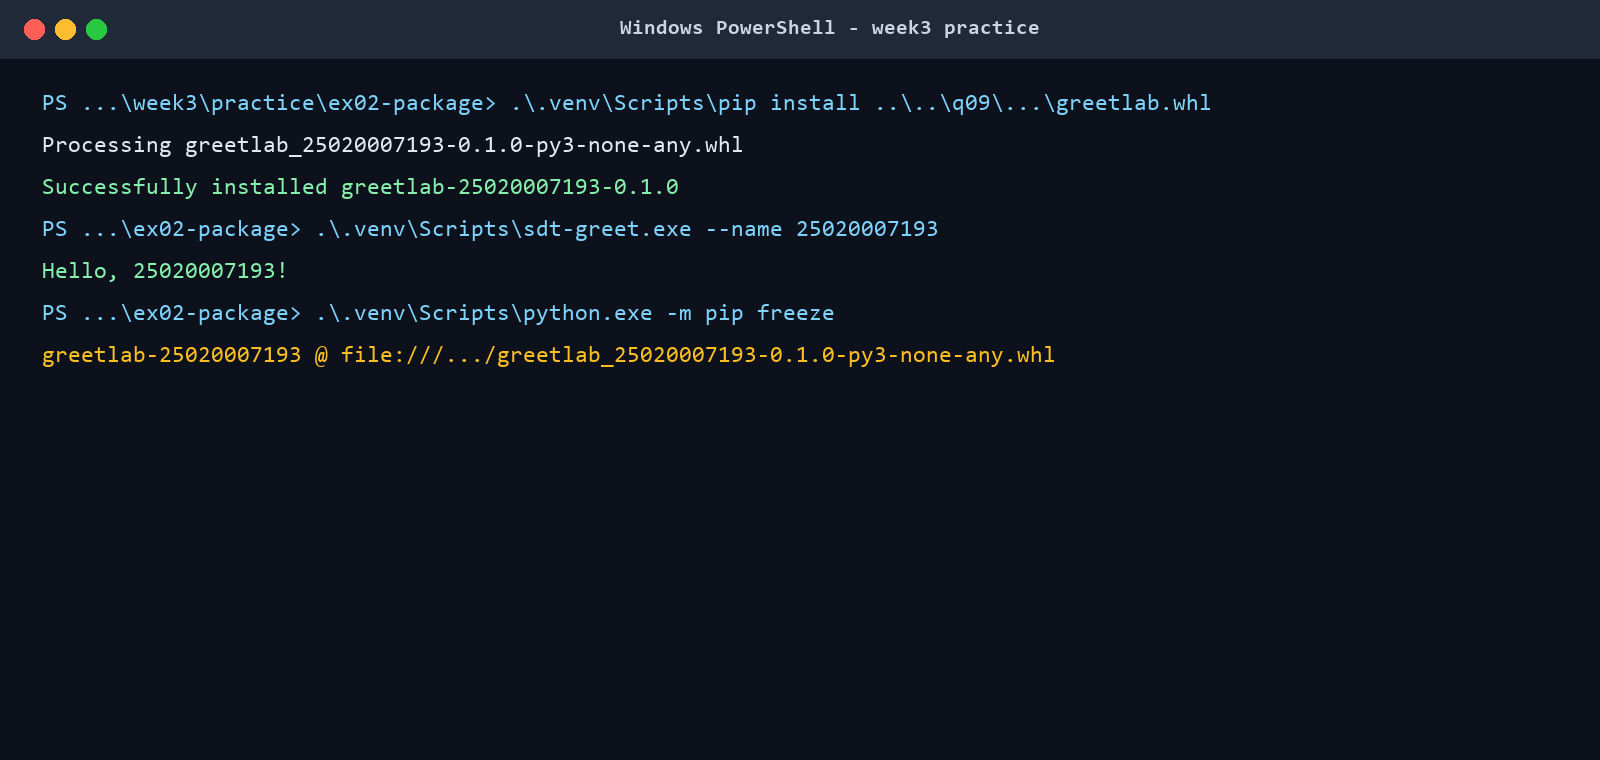
\includegraphics[width=.91\textwidth,height=.39\textheight,keepaspectratio]{assets/practice-ex02-wheel.png}
  \caption{实例 2 本地 Wheel 安装和锁定记录}
\end{figure}

\begin{summarybox}{结果说明}
新建虚拟环境只从实验九生成的 Wheel 安装 \texttt{greetlab-25020007193}，运行入口命令得到
\texttt{Hello, 25020007193!}。生成的 \texttt{requirements.lock} 保留本地 Wheel 路径与
SHA-256 哈希，便于之后复核安装来源。
\end{summarybox}

\clearpage
\practicebanner{3}{为简单 Python 服务编写 Docker 配置}

\subsection*{配置文件}
\begin{lstlisting}[style=shell]
# Dockerfile
FROM python:3.13-slim
WORKDIR /app
COPY app.py .
EXPOSE 8000
CMD ["python", "app.py"]

# docker-compose.yml
services:
  web:
    build: .
    ports: ["8000:8000"]
  cache:
    image: redis:7-alpine
\end{lstlisting}

\begin{summarybox}{结果说明}
在 \texttt{practice/ex03-docker} 中完成单服务 Python HTTP 应用的 Dockerfile，以及包含
\texttt{web} 与 \texttt{cache} 两个服务的 Compose 配置。本机未安装 Docker，因此未把
静态配置误记为容器运行结果；配置可以在具备 Docker 的环境中用
\texttt{docker compose up --build} 继续验证。
\end{summarybox}

\clearpage
\practicebanner{4}{比较四种 AI 辅助编程方式}

\subsection*{体验对比}
\begin{table}[H]
  \centering
  \renewcommand{\arraystretch}{1.30}
  \begin{tabularx}{\textwidth}{p{2.4cm}X}
    \toprule
    方式 & 适用性与观察 \\
    \midrule
    手动编码 & 对接口、约束与细节控制最强，适合需要深入理解或关键逻辑。 \\
    AI 自动补全 & 适合已明确下一段代码时减少重复输入，但仍需人工审查上下文。 \\
    内联聊天 & 适合局部解释、重命名和小范围重构，便于保持当前编辑位置。 \\
    编程智能体 & 适合可运行测试的多文件任务；实验十展示了“失败测试--修复--复测”的反馈闭环。 \\
    \bottomrule
  \end{tabularx}
\end{table}

\begin{summarybox}{结果说明}
四种方式并非互相替代。对本周的空白名称缺陷，智能体能够执行测试、定位失败并提交最小修复；
但测试目标、diff 审查与最终结论仍由人工把关。
\end{summarybox}

\clearpage
\practicebanner{5}{让智能体阅读陌生的 greetlab 包}

\subsection*{阅读路径}
\begin{lstlisting}[style=shell]
rg --files week3/q09/q09
Get-Content week3/q09/q09/pyproject.toml
Get-Content week3/q09/q09/src/greetlab/cli.py
\end{lstlisting}

\begin{summarybox}{结果说明}
从 \texttt{pyproject.toml} 可知项目名为 \texttt{greetlab-25020007193}，
\texttt{project.scripts} 将 \texttt{sdt-greet} 映射至
\texttt{greetlab.cli:main}。再读取 \texttt{cli.py} 可确认它使用 argparse 读取
\texttt{--name} 并输出问候语。该练习说明先建立入口、包结构和行为的整体图，再修改代码更稳妥。
\end{summarybox}

\practicebanner{6}{氛围编程一个小型问候页}

\subsection*{产物}
\begin{lstlisting}[style=shell]
start week3\practice\ex06-vibe-greeting\index.html
\end{lstlisting}

\begin{summarybox}{结果说明}
由编程智能体生成的单页应用保存在 \texttt{ex06-vibe-greeting/index.html}。页面提供姓名输入框与
按钮：非空输入显示问候语，空输入提示“请输入非空姓名”。该实例的重点是用自然语言描述目标并
检查生成产物，而不是手工逐行编写页面代码。
\end{summarybox}

\clearpage
\practicebanner{7}{不直接编辑 Markdown，提取无序列表}

\subsection*{执行命令}
\begin{lstlisting}[style=shell]
rg -N '^\s*-\s+' input.md > list-items.txt
Get-Content list-items.txt
\end{lstlisting}

\begin{figure}[H]
  \centering
  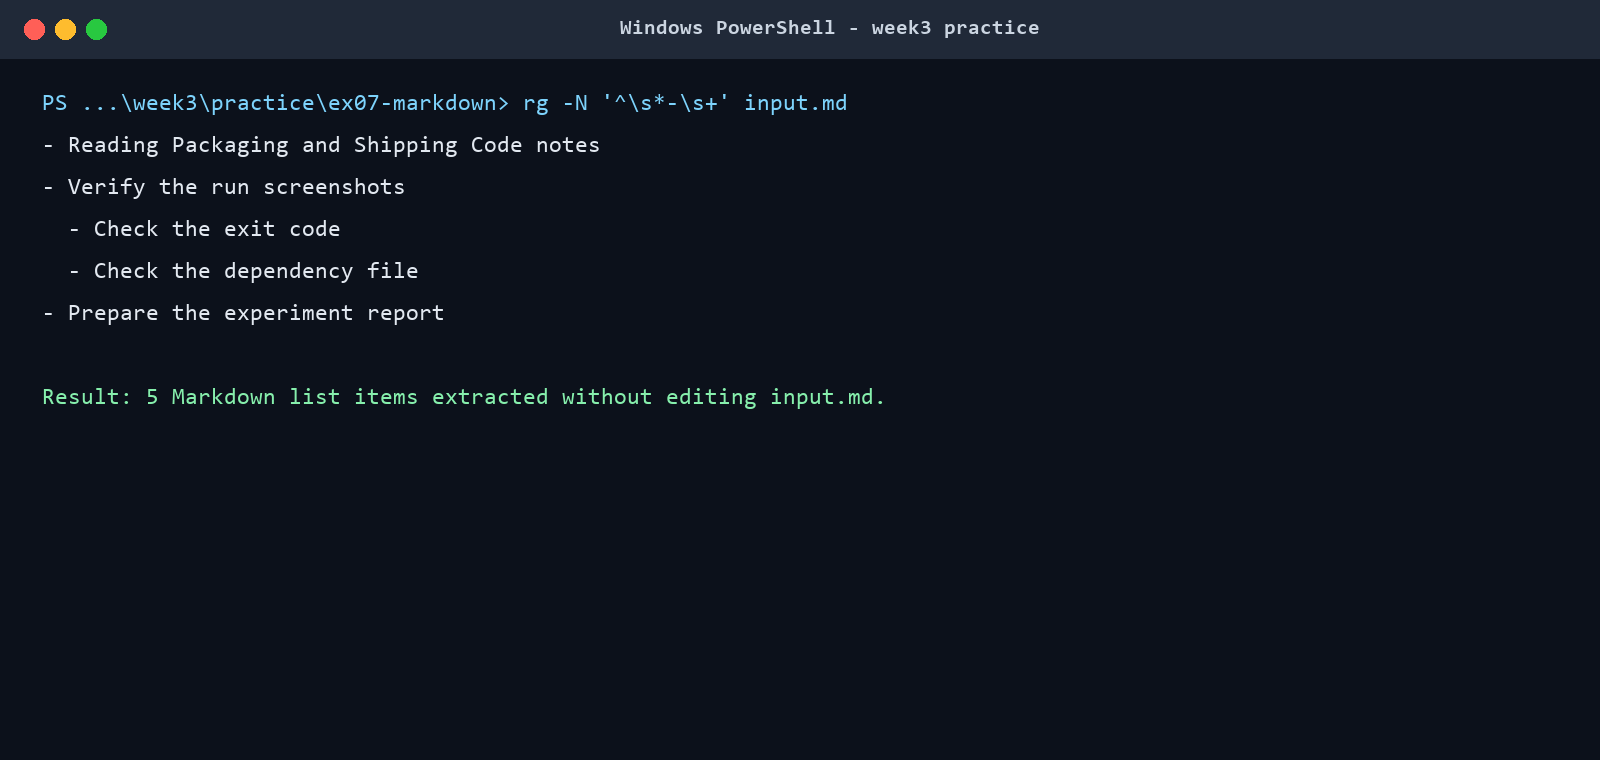
\includegraphics[width=.91\textwidth,height=.39\textheight,keepaspectratio]{assets/practice-ex07-rg.png}
  \caption{实例 7 使用 rg 提取 Markdown 无序列表}
\end{figure}

\begin{summarybox}{结果说明}
命令直接从 \texttt{input.md} 中匹配带可选缩进的无序列表行，得到 5 个项目，其中包括
两项嵌套列表。原 Markdown 文件未被编辑，结果单独写入 \texttt{list-items.txt}。
\end{summarybox}

\clearpage
\practicebanner{8}{比较仓库中的提交信息}

\subsection*{执行命令}
\begin{lstlisting}[style=shell]
git show -s --format='%h%n%s%n%b' e1a47a8
git show -s --format='%h%n%s%n%b' 9983913
\end{lstlisting}

\begin{figure}[H]
  \centering
  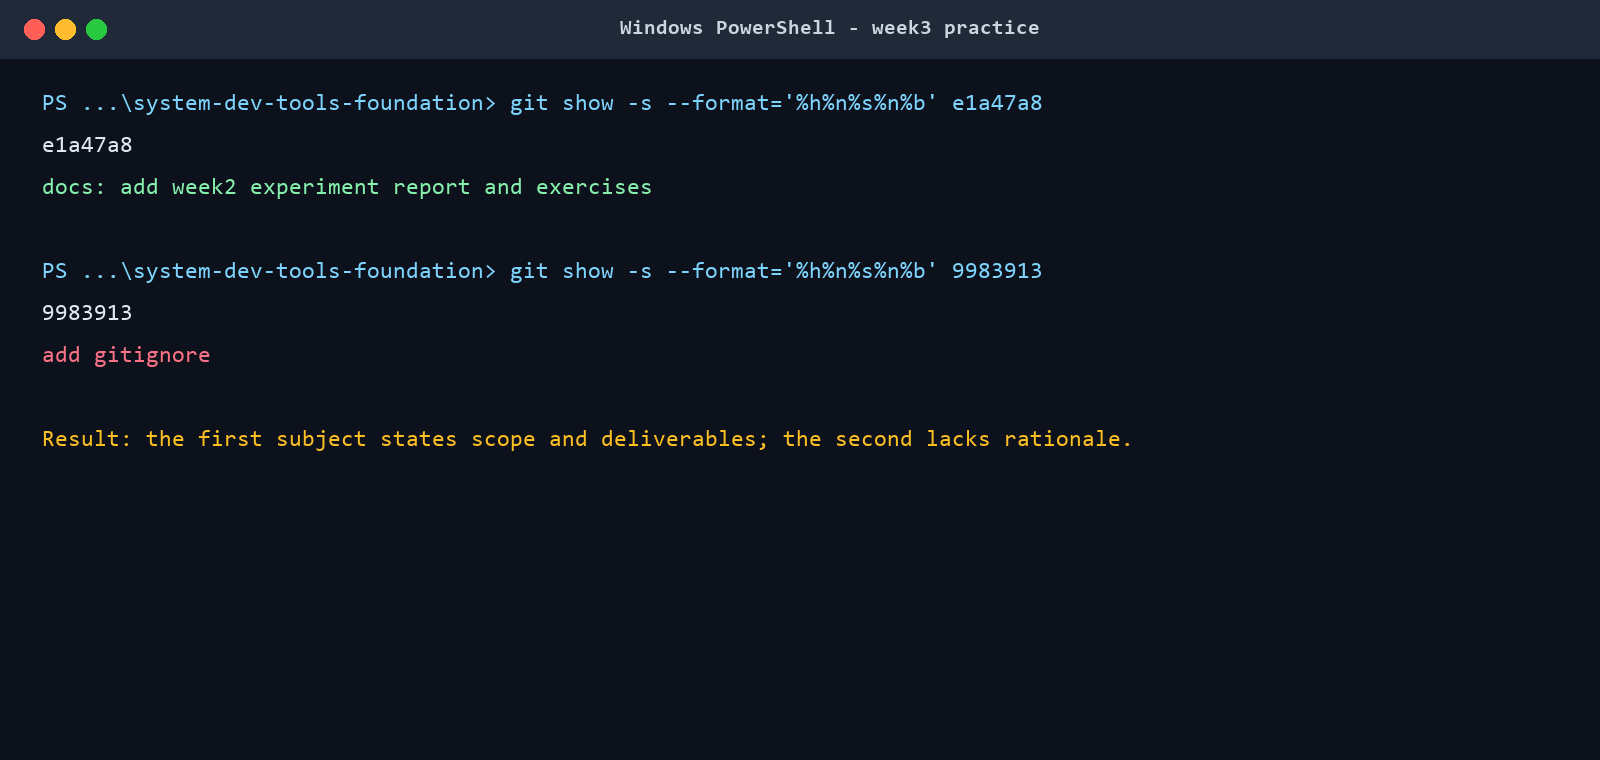
\includegraphics[width=.91\textwidth,height=.39\textheight,keepaspectratio]{assets/practice-ex08-git.png}
  \caption{实例 8 Git 提交信息对比}
\end{figure}

\begin{summarybox}{结果说明}
\texttt{docs: add week2 experiment report and exercises} 指明了修改范围和交付物；
\texttt{add gitignore} 则缺少为何忽略、忽略哪些文件的背景。改进版提交信息与完整分析保存在
\texttt{practice/ex08-git-history.md}。
\end{summarybox}

\clearpage
\practicebanner{9}{用 q10 缺陷构造最小可复现示例}

\subsection*{复现与验证}
\begin{lstlisting}[style=shell]
python -m unittest discover -s tests -v
python -c "import sys; sys.path.insert(0, 'src'); \
from greetlab.cli import main; \
sys.argv=['sdt-greet','--name','   ']; main()"
echo $LASTEXITCODE
\end{lstlisting}

\begin{summarybox}{结果说明}
最小示例只保留 \texttt{greetlab}、一个全空格的 \texttt{--name} 参数与对应测试。修复前，
测试断言 \texttt{SystemExit} 未抛出；修复后，argparse 报错且退出码为 \texttt{2}。这正是
将复杂问题剥离为可稳定复现案例的价值。
\end{summarybox}

\practicebanner{10}{对比三个开源项目的 README}

\subsection*{对比结果}
\begin{table}[H]
  \centering
  \renewcommand{\arraystretch}{1.30}
  \begin{tabularx}{\textwidth}{p{2.0cm}X}
    \toprule
    项目 & README 的信息组织与可借鉴点 \\
    \midrule
    FastAPI & 首屏给出用途与核心特性，随后提供安装、可运行示例和文档入口。 \\
    Requests & 以简短用途、安装和最常见调用路径为主，读者可快速开始。 \\
    Rich & 先展示终端视觉效果，再按功能、安装和文档链接展开，降低理解门槛。 \\
    \bottomrule
  \end{tabularx}
\end{table}

\begin{summarybox}{结果说明}
三个 README 都先回答“它做什么”“为什么值得使用”“如何开始”，随后才引向深入文档。
完整对比记录在 \texttt{practice/ex10-readme-comparison.md}。该漏斗式组织方式可用于后续整理
自己的项目说明。
\end{summarybox}

\vspace{0.65cm}
\begin{summarybox}{解题感悟}
本周实验让我进一步理解了可交付软件不仅需要实现功能，也需要可靠的打包验证、可复现的
测试、清晰的协作信息和可核验的训练结果。对失败过程、修复范围和最终输出进行记录，
能够让问题定位与后续复查更直接、更可信。
\end{summarybox}

\vspace{0.55cm}
\begin{summarybox}{GitHub 仓库}
\centering
\url{https://github.com/FinaleQuill/system-dev-tools-foundation.git}
\end{summarybox}

\end{document}
